\section{Geschäftsidee}


\subsection{Worum es hier geht}
Eine Studie von International Data Corporation (IDC, eines der führenden Marktforschungs-unternehmen in der IT-Industrie) aus dem Jahr 2005\footnote[1]{\textit{White Paper on Hidden Cost of Information Work}, IDC, 2005.} hat gezeigt, dass ein Wissensarbeiter im Durchschnitt rund ein Viertel seiner Arbeitszeit alleine auf die Informationssuche aufwendet. In der wissenschaftlichen Forschung ist dieser Anteil unseren Schätzungen zufolge noch größer. Gesucht wird dabei vor allem nach Information in Form von wissenschaftlichen Publikationen. Weil Publikationen im Idealfall den Stand der Technik abbilden, ist deren Studium ein Grundpfeiler erfolgreicher wissenschaftlicher Praxis. 

\begin{table}[h!]
  \centering
  \begin{large}
	\begin{itshape}
  \begin{tabular}{c}\hline
	\\
  {\color{orange}„Wenn ich weiter geblickt habe, so deshalb,} \\ 
	{\color{orange}weil ich auf den Schultern von Riesen stehe.“} \\
	{\hfill \color{orange}\textit{Isaac Newton, 1676} } \\
	\\\hline
  \end{tabular}
	\end{itshape}
  \end{large}
\end{table}

Neben den obligatorischen Veröffentlichungen in Journals und Konferenzbändern bergen Blogs und Magazine häufig eine nicht minder wichtige Quelle für neue Ideen und Herangehensweisen. An dieser Stelle kommen allerdings vier wichtige Faktoren ins Spiel, die eine erfolgreiche Literaturrecherche erheblich erschweren: 

\begin{description}
  \item[\textbf{\color{orange}{Informationsuniversum wächst:}}] \hfill \\
  Die Zahl möglicher Quellen und potentiell wertvoller Informations-Items wächst rasant: 
In 2008 erschienen allein in den neun\footnote[2]{Nach UNESCO Science Report 2010: GER, FRA, UK, RUS, JPN, KOR, CHN, CAN, USA} großen Wissenschaftsnationen 760.671 Veröffentlichungen. Bei der gegenwärtigen jährlichen Wachstumsrate von 3,26\% wird sich diese Zahl in zwanzig Jahren verdoppeln. 
  \item[\textbf{\color{orange}{Information veraltet:}}] \hfill \\
  Neu produziertes Wissen veraltet heute schneller als jemals zuvor. Neue Entwicklungen in einem Forschungsfeld werden schnell entdeckt, aufgegriffen und weiterentwickelt. Wenn man Fortschritt erzielen möchte, ist jede Verzögerung bei der Informationssuche ein schwerwiegender Nachteil. 
  \item[\textbf{\color{orange}{Wissensgebiete werden vernetzt:}}] \hfill \\
  Die Grenzen zwischen den Disziplinen verschwimmen zunehmend. Bahnbrechende Arbeiten über Datenverarbeitung werden manchmal in Biologie-Journals publiziert, weil beispielsweise die Genomforschung ohne Informatik nicht mehr auskommt. Solche potentiell interessanten Informations-Events bleiben natürlich unentdeckt, wenn man die Aufmerksamkeit unmittelbar auf das eigene Feld beschränkt. 
 \item[\textbf{\color{orange}{Verfügbare Such-Tools sind unzulänglich:}}] \hfill \\
	Die Möglichkeiten der Suche in der globalen Informationswolke, bereitgestellt durch Incumbents wie Google und Microsoft, sind weitgehend auf Schlüselworte beschränkt. Dabei ist die Suche nach Bedeutungs-Nuancen und Konzepten das, was eine effektive Literaturrechere ausmacht. 
\end{description} Diese Probleme wird \textsc{\color{orange}{SemLit}} lösen. Mit semantischen Technologien werden wir die Praxis der Literaturarbeit umkrempeln. Im Folgenden beschreiben wir, wie das im Detail geschehen soll. 

\begin{table}[h!]
  \centering
  \begin{large}
	\begin{itshape}
  \begin{tabular}{c}\hline
  \\
  {\color{orange}Ein Wissensarbeiter verbringt durchschnittlich }\\
  {\color{orange}24\% seiner Zeit mit Informationssuche.}\\
  \\\hline
  \end{tabular}
	\end{itshape}
  \end{large}
\end{table}


%=======================================

\subsection{Know-how Träger}
Die Idee und Umsetzung wird von zwei Studenten des Karlsruher Instituts für Technologie (KIT) entwickelt. {\color{orange}Artem Schumilin} studiert Wirtschaftsingenieurwesen (M.Sc) und {\color{orange}Igor Tseyzer} studiert Informationswirtschaft (B.Sc). Während des Studiums am KIT haben beide Gründer die notwendigen Kenntnisse in Web- und Semantic-Web-Technologien gesammelt, was als stabiles Fundament für den Aufbau und weitere Entwicklung der Firma dienen soll. 
\begin{figure}[h!]
\centering

\includegraphics[width=0.6\textwidth]{jsi-aifb-logo}
\end{figure}
\emph{<hier: Liste relevanter Fähigkeiten und Erfahrungen>}
Igor wird im neuen Unternehmen die Marketingstrategie entwickeln und den Vertrieb organisieren, während Artem Verantwortung für die Produktentwicklung und die Finanzen übernehmen wird. 
\\
\\
Neben dem KIT-eigenen Gründernetzwerk stehen den Gründern renommierte Partner aus der Forschung zur Seite: 
Das Josef-Stefan-Institut (JSI) hat mit \emph{Enrycher} die weltweit führende \emph{named entity recognition engine} entwickelt und tritt damit als der Tchnologiepartner von SemLit auf. 
Das Institut AIFB des KIT erweist sich als erfahrener Mentor in Sachen Ausgründung im Bereich semantischer Technologie und wird das Start-Up mit seinen Kontakten und Rat unterstützen.

%=======================================

\subsection{Innovation}

\textsc{Schritt 0:} wo es beginnt\\
Wir beginnen bei den Informations-Items, die im Internet zur freien Verfügung stehen. Dazu gehören vor allem die Abstracts von wissenschaftlichen Veröffentlichungen aus Journals und Konferenzbänden aber auch Artikel in relevanten Blogs und Online-Magazinen. Die Vielzahl der Quellen wird automatish überwacht, um die Nahezu-Echtzeit-Anforderung erfüllen zu können.\\
{\color{orange}Unsere Kunden können die Auswahl der Quellen auf ihre individuellen Bedürfnisse anpassen. }
\\
\\
\textsc{Schritt 1:} die Semantik hinter dem Text\\
Der Kerngedanke hinter SemLit gründet auf den Möglichkeiten, die durch semantische Repräsentation von Textinformation entehen. Dazu gehört die Erkennung von named entities und ihrer Beziehungen untereinander. Mit JSI's Enrycher steht uns die derzeit weltbeste Technologie bereit, mit deren Hilfe wir die Extraktion semantischer Information aus Textdokumenten realisieren. 
\\
\begin{figure}[h!]
\centering
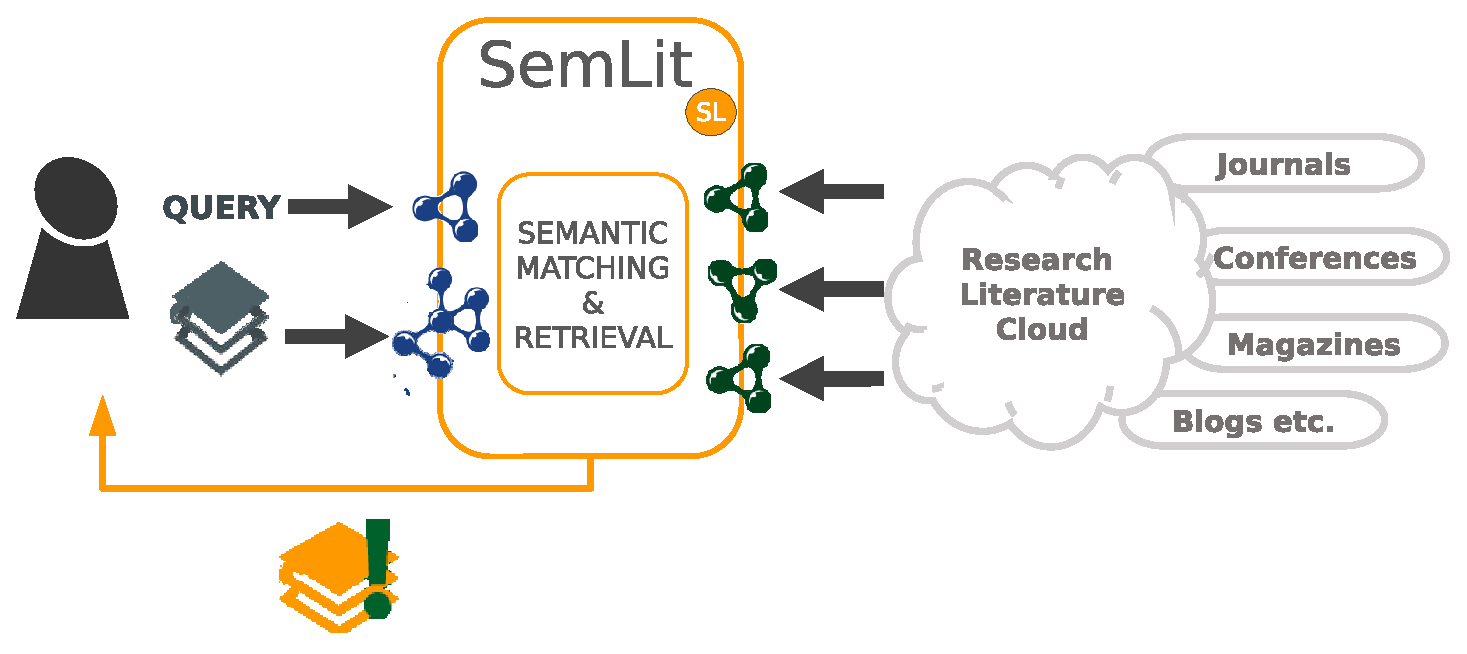
\includegraphics[width=0.9\textwidth]{idea}
\caption{Funktionsschema von SemLit}
\label{fig:idea}
\end{figure}
\\
\textsc{Schritt 2: Informationswunsch äußern}\\
Wie die Textinformation auf der einen Seite, können auf der anderen Seite auch die Suchanfragen der Kunden semantisch repräsentiert werden. Damit kann der Benutzer extrem nuancierte Konzepte ausdrücken. 
Dieses semantische \emph{information retrieval} liefert deutlich bessere Ergebnisse als die gewöhnliche Schlüsselwortsuche alleine. Schlüsselworte sind oft mehrdeutig und liefern damit irrelevante Suchergebnisse, die unnötig Zeit kosten. \\
{\color{orange}Bei SemLit sucht der Benutzer nicht nach einem Wort, sondern nach dem Sinn, der hinter diesem Wort steckt.}
\\
\\
\textsc{Schritt 3: wir gehen weiter als die Anderen}\\
Wir bleiben keineswegs bei den Suchanfragen stehen, sondern gehen noch einen Schritt weiter: Nichts sagt mehr über das Suchinteresse eines Benutzers aus als seine bestehende Dokumentensammlung. Warum also nicht daraus lernen? --- Bei SemLit hat der Kunde die Möglichkeit, ein individuelles System durch Hochladen eigener Dokumente zu trainieren.
\\
\\
{\color{orange}Unter dem Strich entsteht eine Webplattform zur automatischen und individuellen Überwachung der Informationslandschaft. Das System weiß, was der Benutzer will und informiert ihn rechtzeitig, wenn die passende Publikation, ein Blogeintrag oder News-Artikel im Web auftauchen.}

%=======================================

\subsection{Produkt}
SemLit soll in Form einer Web-Applikation und einer App für mobile Geräte an die Kunden ausgeliefert werden. In den nachfolgenden Abbildungen \ref{fig:app} und \ref{fig:website} erklären Entwürfe die wichtigsten Komponenten der Funktionalität. 
\\
\begin{figure}[h!]
\centering
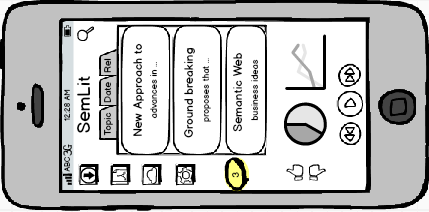
\includegraphics[width=0.5\textwidth]{app}
\caption{SemLit mobile App aggregiert die Funktionalität des Webportals auf kleinem Raum.}
\label{fig:app}
\end{figure}
\\
\\
\\
\begin{figure}[h!]
\centering
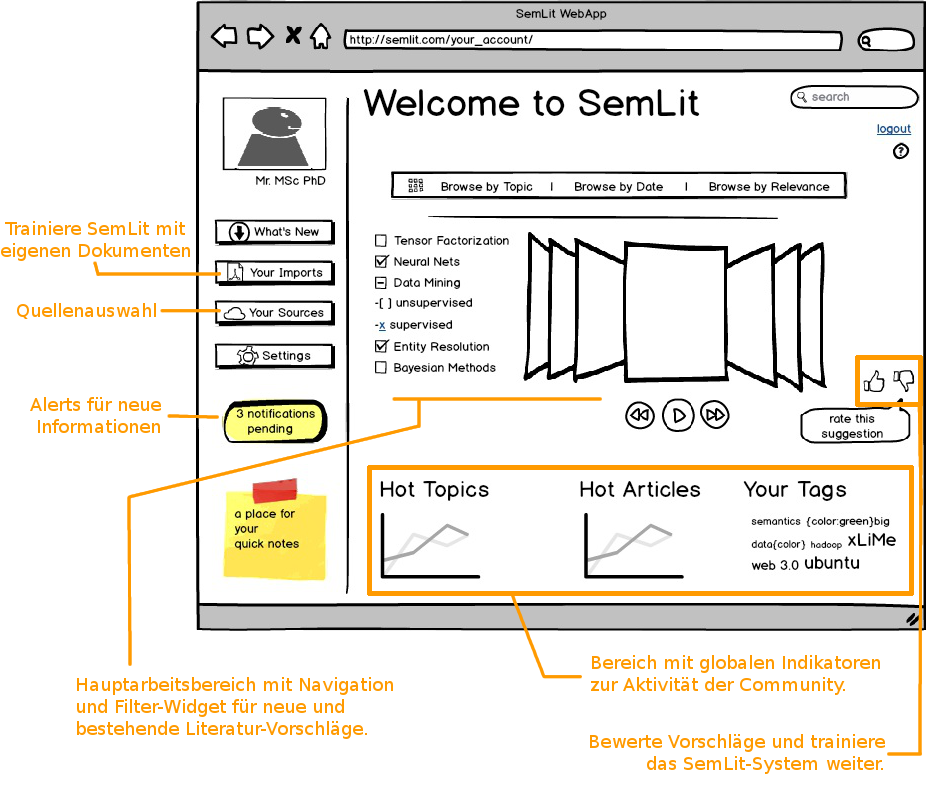
\includegraphics[width=1\textwidth]{website}
\caption{SemLit Webportal mit Erläuterungen zu den wichtigsten Komponenten der Funktionalität.}
\label{fig:website}
\end{figure}

\newpage
%=======================================

\subsection{Customer Value Proposition}
Das Problem mühsamer und zeitraubender Literaturrecherche besteht schon seit es wissenschaftliches Arbeiten gibt. SemLit ist der erste Service auf dem Markt, der dieses Problem durch weitgehende Automatisierung mit semantischen Technologien löst. 
\\
Eine regelbare Vielzahl an Quellen wird durch ein lernfähiges System analysiert und überwacht. Durch SemLit ergeben sich also konkrete Vorteile für den Kunden:
\begin{itemize}
\item Hohe Qualität der Suchergebnisse durch Semantik
\item Neue, potentiell interessante Ergebnisse aus angrenzenden Fachgebieten werden mitgeliefert
\item Informationssuche wird automatisiert
\item Nahezu-realtime Benachrichtigung über neue Veröffentlichungen
\item System passt sich dem Benutzer durch Lerneffekte an und wird mit der Zeit noch besser
\end{itemize}

Die Verbesserung aus diesen Faktoren lässt sich wiederum in Zahlen fassen: Wenn man auf die zuvor erwähnte Studie des IDC (2005) zurückgreift, kann ein Wissensarbeiter demnach mindestens 25\% seiner Zeit einsparen, indem er die Informationssuche mit SemLit weitgehend automatisiert. Für den Arbeitgeber bedeutet das eine geldwerte Ersparnis in Höhe von über 10.000\euro{}  pro Jahr\footnote[4]{Ausgehend vom bundesweiten monatlichen Durchschnittsgehalt von 3.600\euro{}  brutto.}. 

%=======================================


\subsection{Unternehmensplanung}

\subsubsection{Rechtliches}
Das Gründerteam wählt die mini-GmbH als Rechtsform für die Anfangsphase der Unternehmung. Vorteile davon sind die geringeren Kosten der Anmeldung und Anfangsfinanzierung. Im Laufe der nächsten zwei Jahre wird durch periodische Einstellungen ins Eigenkapital die Rechtsform der vollwertigen GmbH erreicht. 
\\
Beide Gründer sind Gesellschafter und nehmen die Verantwortung ebenfalls zu gleichen Teilen als Geschäftsführer wahr.

%=======================================

\subsubsection{Meilensteine}
Wir identifizieren fünf wichtige Events und Prozesse innerhalb der ersten zwei Jahre nach der Gründung. Sie sind auch deshalb bedeutend, weil sie als Umbruchpunkte im Finanzplan behandelt und abgebildet werden.\\
\begin{description}
  \item[\textbf{1. Offizieller Start}] \hfill \\
In den ersten Wochen sollen vor allem die rechtlichen Einzelheiten geregelt werden. Das wird mit kompetenter Begleitung des Centers für Innovation und Entrepreneurship (CIE) des KIT erfolgen. Das CIE verfügt über Erfahung in diesem Bereich und kann den Kontakt zu bewährten Steuerberatern, Anwälten und weiteren wichtigen Ansprechpartnern empfehlen. In dieser Phase sollen die Anmeldung des GmbH-Sitzes, die Re-gistrierung und Eintragung der GmbH ins Handelsregister vorgenommen werden. 
\\
  \item[\textbf{2. Produktionsgrundlage}] \hfill \\
Damit die nachfolgende Produktentwicklung einsetzen kann, müssen die Rechenkapa-zitäten und Lizenzen erworben werden. Die Rechenkapazitäten werden kostengünstig und flexibel bei {\color{orange}Amazon Web Services} eingekauft. Das Gründerteam verfügt bereits über praktische Erfahrung im Umgang mit dem IaaS-Angebot von Amazon und kann diese Technologien gut einschätzen. 
\\
Der zweite wichtige Teil dieser Phase umfasst den Erwerb einer Lizenz für \emph{Enrycher}\footnote[3]{Test-Version zu finden als Web-Service unter http://enrycher.ijs.si}, das semantische Textanalyse-Werkzeug des AI-Laboratoriums unseres Technologiepartners JSI. Erster Kontakt zu den Verantwortlichen auf der Seite von JSI konnte über unseren Mentor, das AIFB-Institut, bereits erfolgreich hergestellt werden.
\\
  \item[\textbf{3.1. Produktentwicklung}] \hfill \\
Die ersten 4 Monate nach Kick-Off sind für die Produktentwicklung veranschlagt. Dabei soll die Aufgabe der Frontend-Entwicklung (Infrastruktur und Interface der mobilen Anwendung und der Web-App) an einen geeigneten Dienstleister ausgelagert werden. So kann sich das Gründerteam der Entwicklung der SemLit-Kernkompetenz rund um die Beschaffung, Verwaltung und Analyse der Daten widmen. Damit wird die Time-to-Market signifikant verringert.  
\\
  \item[\textbf{3.2. Marketing \& Kundenaquise}] \hfill \\
Während der letzten Entwicklungsphase werden bereits die ersten Marketing-Kampagnen gestartet. Zunächst sollen verstärkt Privatkunden auf Konferenzen und durch Social-Media-Marketing geworben werden. 
\\
Basierend auf dem Feedback der beta-Kunden werden wir das System verbessern und im Anschluss darauf offensiv um Firmenkunden werben. Zu diesem Zeitpunkt wird ein Kundensupport-Mitarbeiter zum Team stoßen, um eine bessere Betreuung bei Wünschen und Problemen zu gewährleisten.
\\
  \item[\textbf{4. Wachstum}] \hfill \\
Damit das Team adequat die Anregungen und Verbesserungsvorschläge der Benutzer einarbeiten kann, sollte im zweiten Quartal des zweiten Jahres eine feste Developer-Stelle besetzt werden. Das Angebot muss ständig weiterentwickelt und an Kundenwünsche angepasst werden.
\\
  \item[\textbf{5. Break-Even}] \hfill \\
Im Fall von SemLit sind die Kosten der Anfangsphase relativ gut prognostizierbar. Außerdem sind die bedeutsamen Kostenarten (Personal-, Betriebs-, Lizenzkosten) wenig volatil. Damit wird im neutralen Umsatz-Szenario der Break-Even-Punkt schätzungsweise in Q2 des zweiten Geschäftsjahres erreicht. Weitere Details werden im Abschnitt Finanzplanung diskutiert. 
\end{description}

\subsubsection{Abonnement-Pricing}
Die Abonnements sind die vorrangige Quelle für Umsatzerlöse. Im heutigen Marktumfeld ist das Bezahlen für Online-Dienste weit besser angesehen als es noch vor zehn Jahren der Fall war. Deshalb ist bei SemLit folgendes Zahlungsmodell vorgesehen: 
\\
\\
\begin{table}[h!]
  \centering
    \begin{footnotesize}
  \begin{tabular}{|l|l|l|l|}\hline
  \textbf{ } &  \textbf{Private Kunden} &  \textbf{Firmenkunden} \\ \hline
 \textbf{basic version} & 1\euro{} & 150\euro{} \\ \hline
\textbf{extended version} & 3\euro{} & 450\euro{} \\ \hline
  \end{tabular} 
    \end{footnotesize}
  \caption{Preis-Modell für SemLit-Abonnements}
  \label{tab:break-even}
\end{table} 
\\
Die Firmenkunden bezahlen bei diesem Modell unabhängig von der letztendlichen Zahl der Benutzer, was dadurch gerechtgertigt ist, dass die durchschnittliche F\&E-Abteilung als Endkunde meist relativ wenige tatsächliche Benutzer hat.\\
Den Privatkunden kann man die geforderten Entgelte durchaus zumuten, wenn man den gegenwärtigen Micropayments-Markt als Vergleich nimmt: kleine Unterhaltungs-Apps werden im App-Store zu vergleichbaren und größeren Preisen angeboten. Agesichts dessen, dass SemLit ein echtes Produktivitäts-Tool ist, sind die Preise mehr als wettbewerbsfähig. 


